\documentclass[a4paper,12pt]{article}
\usepackage{geometry}
\usepackage{enumitem}
\usepackage{fancyhdr}
\usepackage{xcolor}
\usepackage{sectsty}
\usepackage{multicol}
\usepackage{graphicx}
\usepackage{amsmath}
\usepackage{float}
\def\inputGnumericTable{}
\usepackage[latin1]{inputenc}
\usepackage{fullpage}
\usepackage{color}
\usepackage{array}
\usepackage{longtable}
\usepackage{calc}
\usepackage{multirow}
\usepackage{hhline}
\usepackage{ifthen}
\geometry{top=1in, bottom=1.5cm, left=1.5cm, right=1.5cm}    
\pagestyle{empty}
\sectionfont{\color{blue}}

\begin{document}

\thispagestyle{fancy}
\fancyhf{}
\fancyhead[L]{
    
\includegraphics[width=8cm, height=1.7cm]{IIITB-COMET-Logo.png}
}
\fancyhead[R]{
    Name: N.Srinivas \\
    Batch: COMETFWC036 \\
    Date: 10 September 2025
}
\renewcommand{\headrulewidth}{0pt}
\fancyfoot[C]{\thepage}

\vspace*{1cm}
\begin{center}
    {\LARGE \textbf{\textcolor{blue}{GATE 2010 CS, $9^{th}$ Question Analysis}}}
\end{center}

\section*{Q.9}

\textbf{Question:} The Boolean expression for the output \( f \) of the multiplexer shown below is:
\begin{center}
	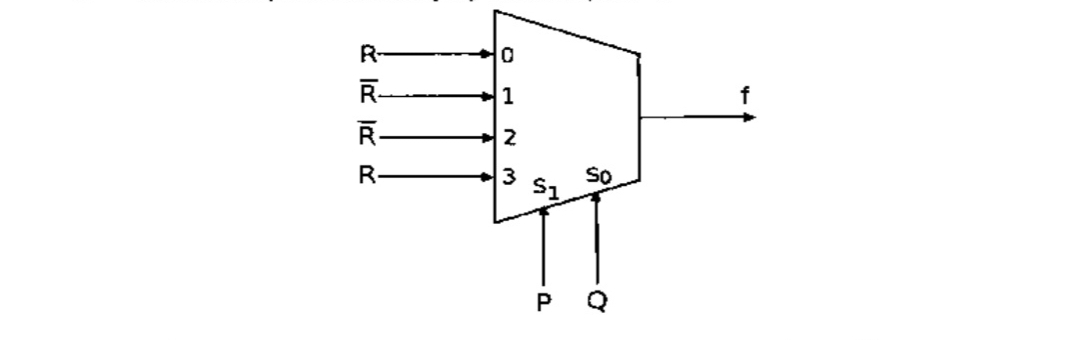
\includegraphics[width=12cm, height=8cm]{circuit.jpg}
\end{center}
\textbf{Options:}
\begin{enumerate}
\item[(A)] \( \overline{P} \oplus Q \oplus R \)
\item[(B)] \( P \oplus Q \oplus R \)
\item[(C)] \( P + Q + R \)
\item[(D)] \( \overline{P + Q + R} \)
\end{enumerate}

\subsection*{Solution:}

The output of a 4:1 multiplexer is:

$
f = I_0 \cdot \overline{P} \cdot \overline{Q} + I_1 \cdot \overline{P} \cdot Q + I_2 \cdot P \cdot \overline{Q} + I_3 \cdot P \cdot Q
$

Substitute the given inputs:

$
I_0 = R,\quad I_1 = \overline{R},\quad I_2 = \overline{R},\quad I_3 = R
$

So,

$
f = R \cdot \overline{P} \cdot \overline{Q} + \overline{R} \cdot \overline{P} \cdot Q + \overline{R} \cdot P \cdot \overline{Q} + R \cdot P \cdot Q
$

\subsection*{Truth Table}

\begin{center}
\begin{tabular}{|c|c|c|c|}
\hline
P & Q & R & f \\
\hline
0 & 0 & 0 & 0 \\
0 & 0 & 1 & 1 \\
0 & 1 & 0 & 1 \\
0 & 1 & 1 & 0 \\
1 & 0 & 0 & 1 \\
1 & 0 & 1 & 0 \\
1 & 1 & 0 & 0 \\
1 & 1 & 1 & 1 \\
\hline
\end{tabular}
\end{center}

This matches the truth table for:

$
f = P \oplus Q \oplus R
$
\section*{\textbf{Hardware Implementation}}
The above problem is implemented and tested in hardware using Arduino UNO board. Here we implemented Sevensegment and blinked the LED as per truth table and verified the expression.
\section*{Required Components \& Pin Connections}
\begin{center}
\begin{minipage}{0.45\textwidth}
\begin{table}[H]
\centering
\begin{tabular}{|c|l|}
\hline
\textbf{S.No} & \textbf{Component} \\ \hline
1 & Arduino Uno Board \\
2 & Breadboard \\
3 & LEDs (1) \\
4 & 7474 IC (1) \\
5 & Resistors: 220$\Omega$ (2) \\
6 & Jumper Wires \\
7 & USB Cable \\
\hline
\end{tabular}
\end{table}
\end{minipage}
\hspace{0.05\textwidth}
\begin{minipage}{0.45\textwidth}
\begin{table}[H]
\centering
\begin{tabular}{|c|c|}
\hline
\textbf{Component} & \textbf{Arduino Pin} \\ \hline
Input P (Q1) & Digital 2 \\
Input Q (Q2) & Digital 3 \\
Input R (Q3) & Digital 4 \\
Output D (7474) & digital 8\\
Output clk(7474) & digital 9\\ 
GND & GND \\
VCC & 5V \\
\hline
\end{tabular}
\end{table}
\end{minipage}
\end{center}
\newpage
\section*{Code Uploading Steps}
\begin{enumerate}
	\item Create a Assembly  project
	\item Write The code in main.c
	\item Run the Assembly project with command "avra filename.asm". It will compile the code and creates .hex file
	\item Copy the .hex file to ArduinoDriod folder
	\item connect the Arduino UNO to mobile with OTG cable
	\item Upload the hex file using "upload precomplied" option
	\item Observe the ouput and verify the expression
\end{enumerate}
\subsection*{Final Answer:}

$
\boxed{f = P \oplus Q \oplus R}
$

\end{document}
